\documentclass{article}
\usepackage{amsmath}
\usepackage{graphicx}
\usepackage{animate}
\usepackage{hyperref}
\begin{document}

\title{Hubble's Law in Cosmology}
\author{Rishant Bhagat MM22b052 \\ Github id- rishantbhagat}

\date{\today}

\maketitle

\section{Introduction}
Hubble's law, also known as the Hubble–Lemaître law, states that the farther a galaxy is from Earth, the faster it is moving away from us. This is based on the observation that the light from distant galaxies is redshifted, which means that it has been shifted to longer wavelengths, towards the red end of the visible spectrum. The redshift is caused by the expansion of the universe, which is why distant galaxies are moving away from us.
\begin{figure}[h]
\begin{center}

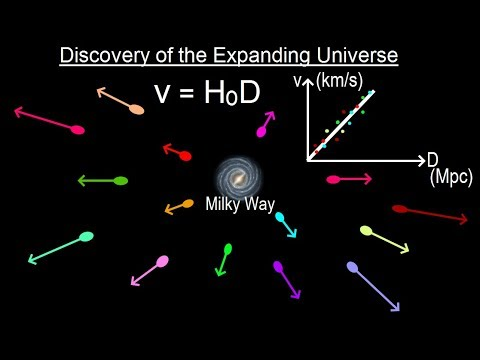
\includegraphics[width=0.5 \textwidth]{hubble.jpg}
\caption{Hubble's law}
\end{center}
\end{figure}
\section{The Equation}
Hubble's law is mathematically represented as:

\begin{equation}
v = H_0 \cdot d
\end{equation}

where $v$ is the recession velocity of a galaxy, $d$ is its distance from Earth, and $H_0$ is the Hubble constant. The Hubble constant represents the rate at which the universe is expanding.
\footnote{\url{https://en.wikipedia.org/wiki/Hubble's_law}}

\section{Interpretation}
Hubble's law states that the recessional velocity of a galaxy is proportional to its distance from Earth. This means that the farther away a galaxy is, the faster it is moving away from us. This is interpreted as evidence that the universe is expanding.

The Hubble constant, $H_0$, is a measure of the rate of expansion of the universe. It is currently estimated to be around $70 \, \text{km} \, \text{s}^{-1} \, \text{Mpc}^{-1}$. This means that for every megaparsec (a unit of distance equal to $3.26 \times 10^{6}$ light-years), galaxies are moving away from us at an average speed of $70 \, \text{km} \, \text{s}^{-1}$.

The Hubble constant is not constant throughout cosmic history. It is thought to have been much higher in the past, and it is likely to continue to increase in the future. This is due to the influence of dark energy, a mysterious form of energy that is thought to make up about 70\% of the universe.\footnote{\url{https://en.wikipedia.org/wiki/Hubble's_law}}

\section{Conclusion}
Hubble's law is a foundational concept in modern cosmology, providing observational evidence for the expanding universe. The equation relating recession velocity to distance, along with the Hubble constant, helps us estimate the age of the universe, study the large-scale structure of galaxies, and explore the nature of cosmic evolution.
\begin{figure}[h]
\begin{center}

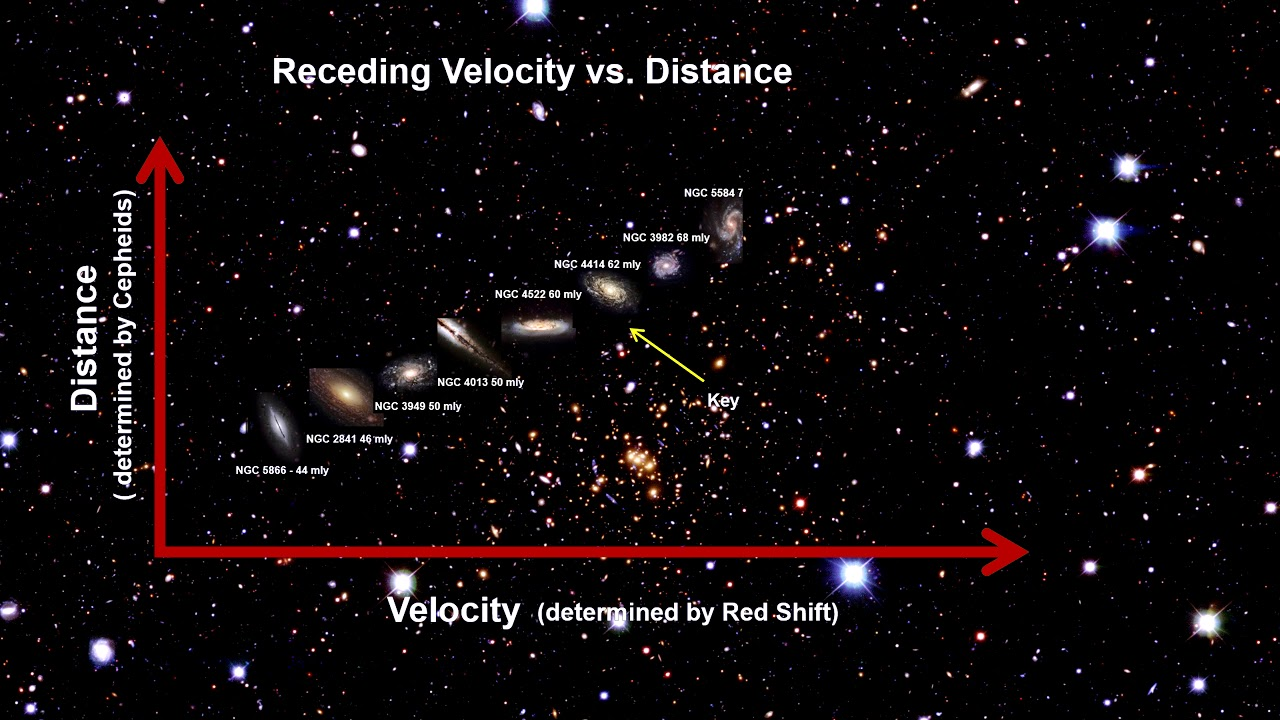
\includegraphics[width=0.7 \textwidth]{maxresdefault.jpg}
\caption{Receding Velocity vs Distance}
\end{center}
\end{figure}




\end{document}